\chapter{Multiscale turbulence measurements}
\label{ch:TurbulenceMeasurements}
Development of a first-principles understanding
of turbulent transport in a tokamak
requires multi-tiered validation\ldots
comparing not just heat fluxes, but
also turbulent spectra etc.
\diiid's extensive suite of fluctuation diagnostics
provides an ideal setting to validate
predicted changes~\cite{howard_pp16}
to turbulent spectra when altering relative drive
between electron-scale and ion-scale turbulence.


\section{Overview of multiscale gyrokinetic predictions}


\section{Experimental conditions}
The experiment was run in the ITER-similar shape,
with aspect ratio, elongation, and triangularity
all closely matched to those of the ITER-baseline scenario
\cite[Sec.~13.5 \& 13.6]{wesson}.
The on-axis toroidal field $B_T = \SI{1.7}{\tesla}$ and
plasma current $I_p = \SI{1.3}{\mega\ampere}$
produced $q_{95} = 3.15$,
where $q_{95}$ is the average value
of the safety factor $q$~\cite[Sec.~3.4]{wesson}
over the surface that encloses $95\%$
of the poloidal flux within the last-closed flux surface.
The neutral beams~\cite[Sec.~5.3-5.5]{wesson}
were operated with feedback to maintain
$\beta_N = 1.9$, where
$\beta_N$ is the normalized plasma pressure~\cite[Sec.~6.18]{wesson}.
In order to suppress core MHD,
an average neutral-beam torque of $\sim \SI{1.5}{\newton \meter}$
was injected into the plasma;
note that this is $\sim 4\times$ larger than
the projected ITER-equivalent torque~\cite{garofalo_nf11}.
In order to alter the local electron-scale and ion-scale drives,
the electron cyclotron resonance heating (ECH)~\cite[Sec.~5.10]{wesson}
location was scanned between $\rho = 0.5$ and $\rho = 0.8$,
where $\rho$ is the square root of the normalized toroidal flux
(which scales as $r / a$, with
$r$ being the minor-radial coordinate and
$a$ being the minor radius of the plasma).
Intra-shot scans of the ECH location
were plagued with core MHD, so
only shot-to-shot, MHD-free scans of the ECH location
are considered here.
The line-averaged density was
$\bar{n}_e = \SI{5.2e19}{\per\meter\cubed}$.
Impurities are removed from the plasma
by both large and small edge localized modes (ELMs)~\cite[Sec.~7.17]{wesson}.
The time histories of several actuators and plasma parameters
are shown in Figure~\ref{fig:TurbulenceMeasurements:traces}.
Note that multiscale gyrokinetic simulations
of this experiment's reference discharge,
\diiid\space shot $153523$ with ECH at $\rho = 0.5$,
indicate that the turbulent transport
is intrinsically multiscale in nature~\cite{holland_nf17}.

\begin{figure}
  \centering
  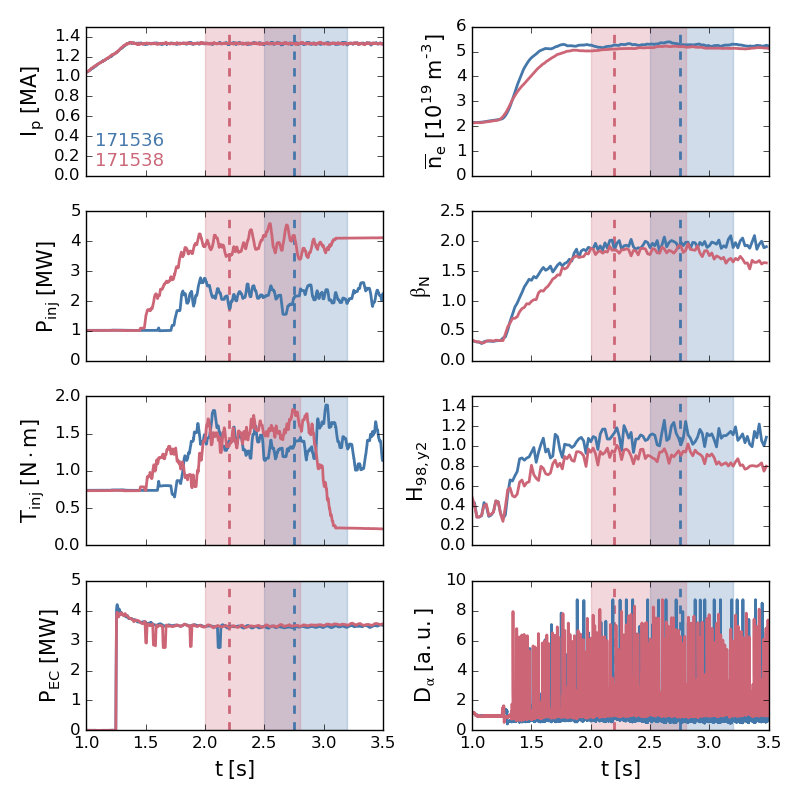
\includegraphics[width = \textwidth]{%
    Chapters/TurbulenceMeasurements/figs/traces.png}
  \caption[Time histories of various actuators \& plasma parameters]{%
    Time histories of various actuators and plasma parameters:
    (a) plasma current $I_p$,
    (b) neutral beam injected (NBI) power $P_{\text{inj}}$,
    (c) NBI torque $T_{\text{inj}}$,
    (d) electron cyclotron resonance heating (ECH) power $P_{\text{ECH}}$,
    (e) line-averaged density $\bar{n}_e$,
    (f) normalized plasma pressure $\beta_N$,
    (g) confinement quality $H_{98,\text{y}2}$, and
    (h) divertor $D_{\alpha}$ light, indicating
    the presence of large and small edge localized modes (ELMs).
    The ECH heating location was
    at $\rho = 0.5$ in $171536$ and
    at $\rho = 0.8$ in $171538$.
  }
\label{fig:TurbulenceMeasurements:traces}
\end{figure}

Equilibrium profiles
\begin{itemize}
  \item averaging over \textcolor{red}{XXX ms}
  \item What types of fits? (splines, RBF, etc.)
  \item Electron-density profiles -- Thomson w/ CO$_2$ normalization?
    Reflectometer?
  \item Electron-temperature profiles -- Thomson \& ECE (or ECE cutoff?)
  \item Ion-temperature profiles -- \textcolor{red}{???}
  \item CER provides C$^{6+}$ density, temperature, and rotation
  \item $E_r$ computed using force balance for
    C$^{6+}$ pressure and toroidal rotation.
    \textcolor{red}{poloidal rotation neglected?}
  \item \textcolor{red}{MSE-constrained EFIT? Kinetic?}
  \item \textcolor{red}{How are ELMs handled?}
  \item Uncertainties
  \item Clear change in turbulent drives with ECH location
\end{itemize}

\begin{figure}
  \centering
  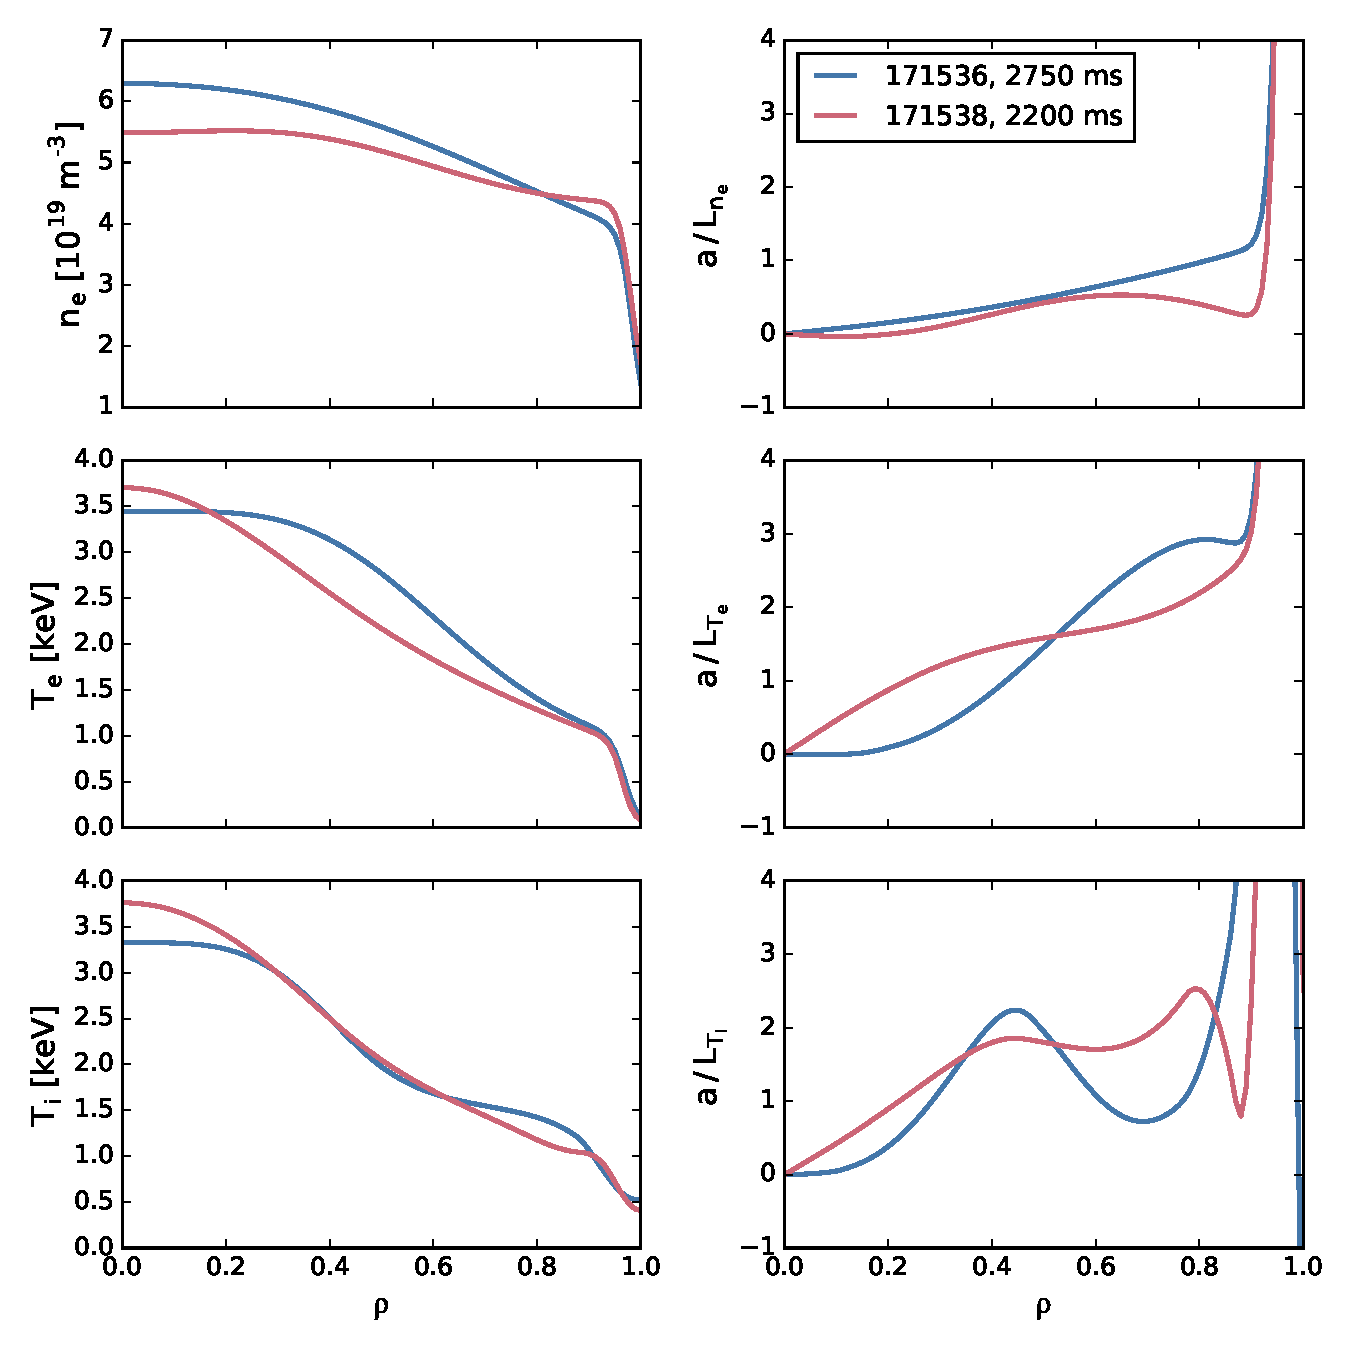
\includegraphics[width = \textwidth]{%
    Chapters/TurbulenceMeasurements/figs/profiles.pdf}
  \caption[Profiles \& inverse scale lengths]{%
    Profiles \& inverse scale lengths from
    OMFIT['TGLF\_scan']['tgyro\_output']
    used as input for TGLF simulations.
  }
\label{fig:TurbulenceMeasurements:profiles}
\end{figure}

\begin{figure}
  \centering
  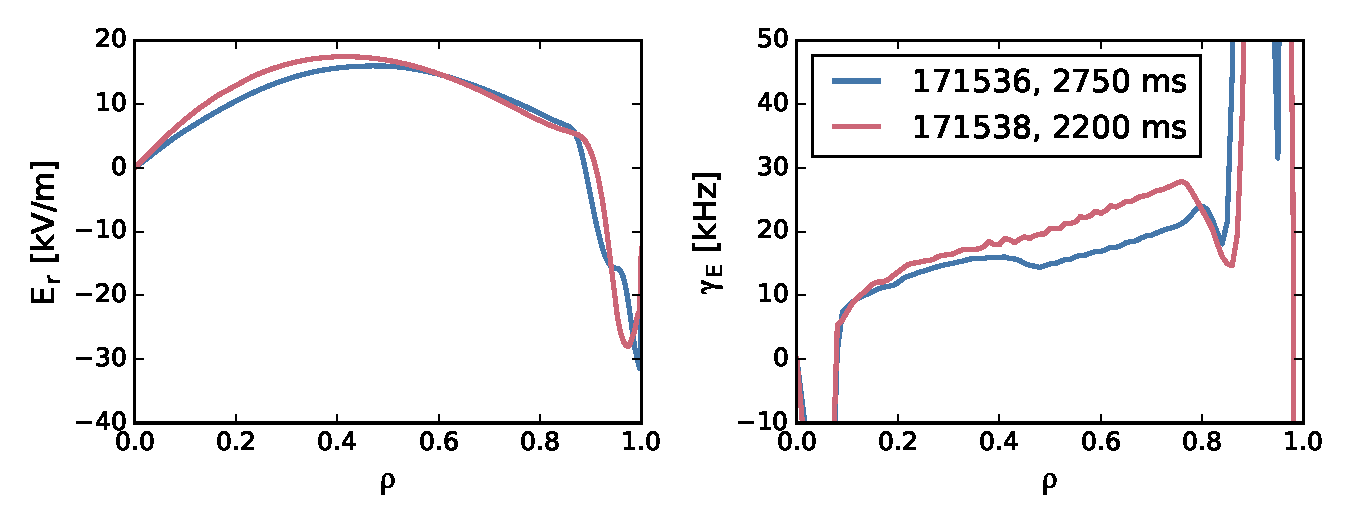
\includegraphics[width = \textwidth]{%
    Chapters/TurbulenceMeasurements/figs/Er_profiles.pdf}
  \caption[Radial electric field \& $E \times B$ shearing rate]{%
    Radial electric field \& $E \times B$ shearing rate from
    OMFIT['TGLF\_scan']['TGYRO']['PROFILES\_GEN']['OUTPUTS']['Er']
    (note that there are no corresponding values from
    OMFIT['TGLF\_scan']['tgyro\_output']
    from which Figure~\ref{fig:TurbulenceMeasurements:profiles}
    was generated, which is why this is a separate figure\ldots).
  }
\label{fig:TurbulenceMeasurements:Er_profiles}
\end{figure}


\section{Measurements}
\begin{figure}[h!]
  \centering
  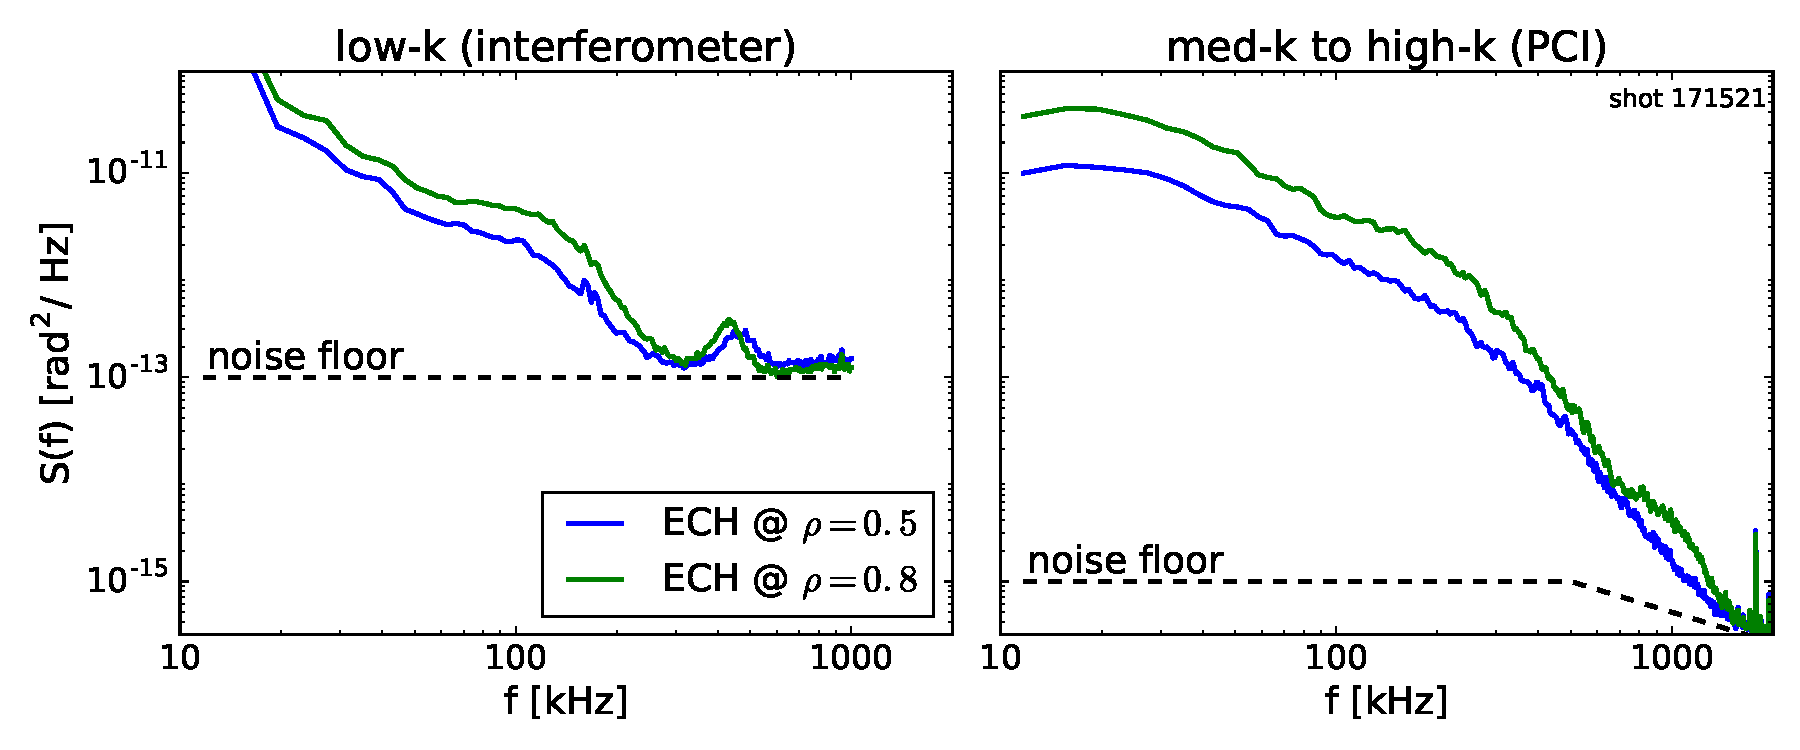
\includegraphics[width = 0.9 \textwidth]{%
    Chapters/TurbulenceMeasurements/figs/spectra_171521_quarterly_review.pdf}
  \caption[Combined PCI-interferometer measured spectra]{%
    Combined PCI-interferometer measured spectra.
  }
\label{fig:TurbulenceMeasurements:spectra_quarterly_review}
\end{figure}

\begin{figure}[h!]
  \centering
  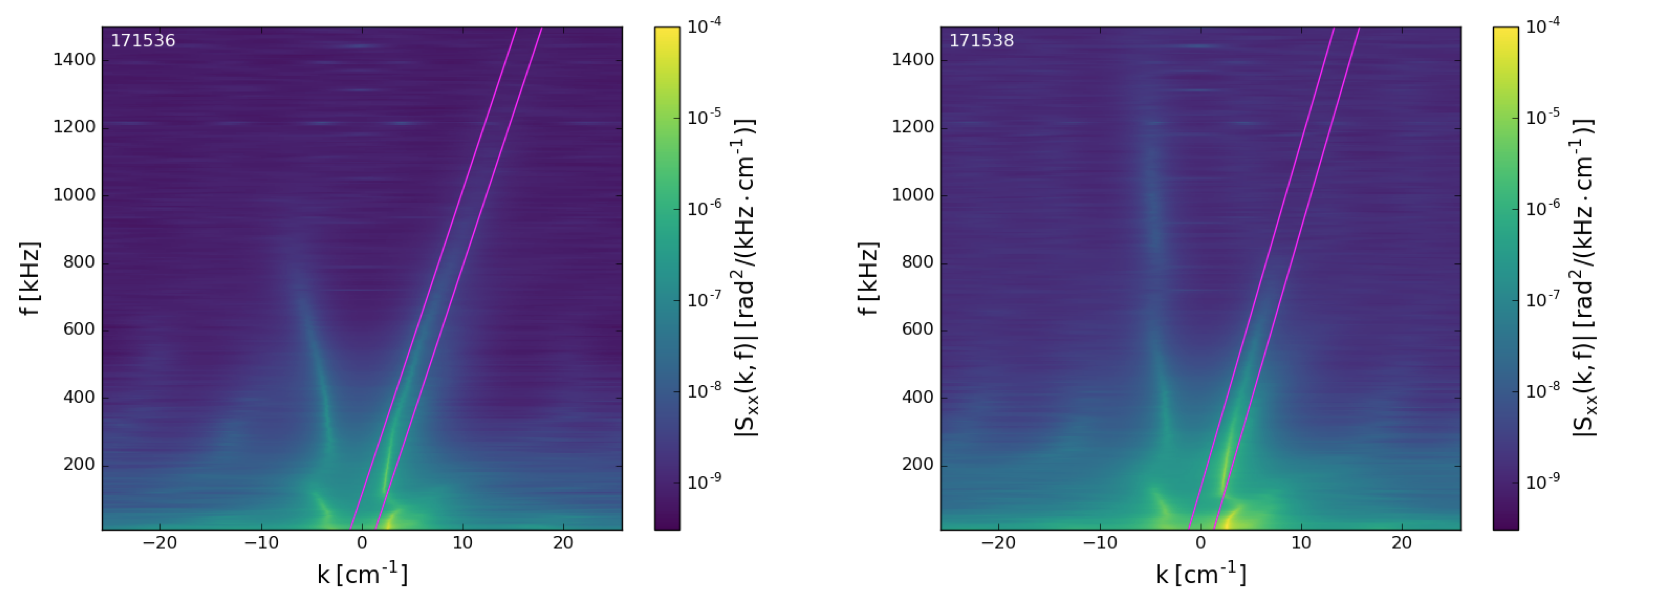
\includegraphics[width = \textwidth]{%
    Chapters/TurbulenceMeasurements/figs/Skf_annotated.png}
  \caption[PCI-measured $S(k, f)$ with branch annotations]{%
    PCI-measured $S(k, f)$ with branch annotations.
  }
\label{fig:TurbulenceMeasurements:Skf_annotated}
\end{figure}

\begin{figure}[h!]
  \centering
  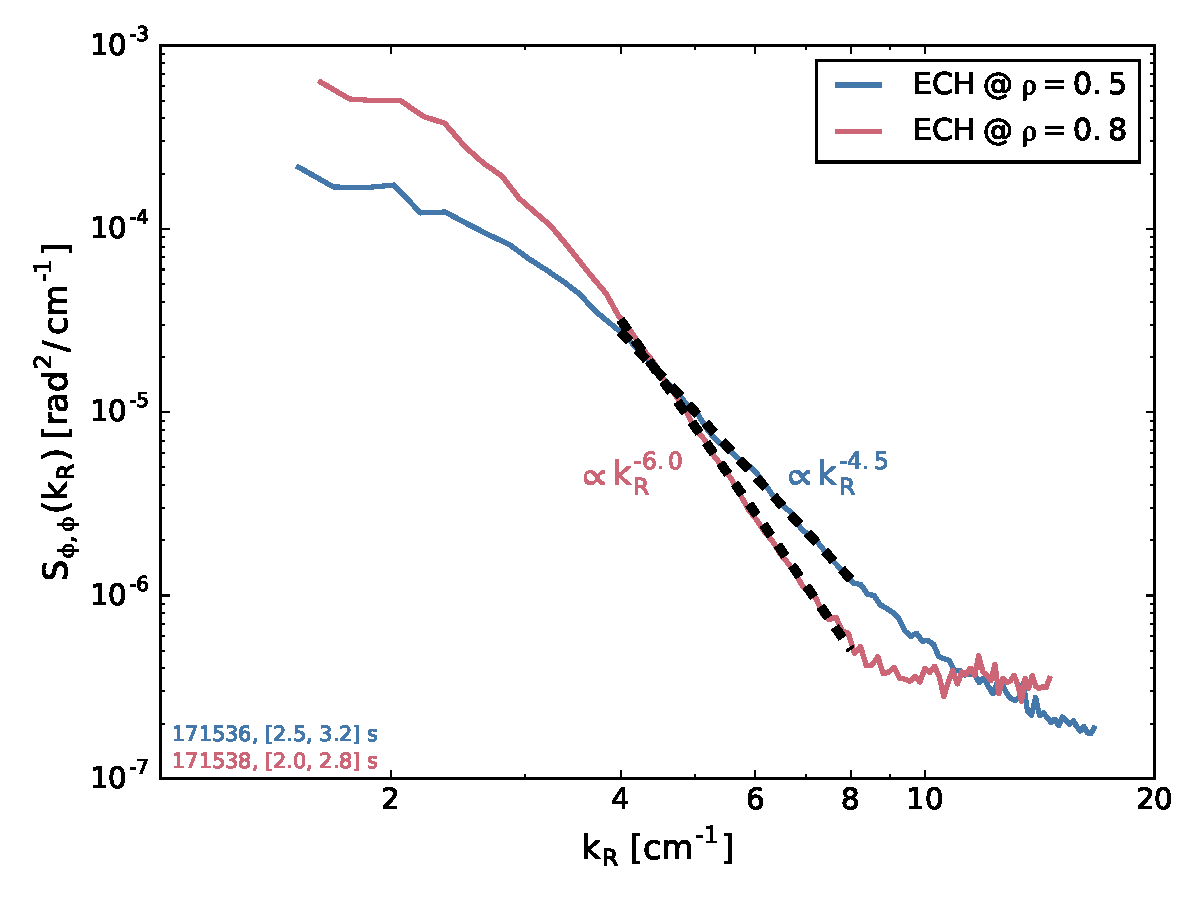
\includegraphics[width = 0.6 \textwidth]{%
    Chapters/TurbulenceMeasurements/figs/Sk_power_law.pdf}
  \caption[PCI-measured power law]{%
    PCI-measured power law from branches annotated in
    Figure~\ref{fig:TurbulenceMeasurements:Skf_annotated}.
  }
\label{fig:TurbulenceMeasurements:Sk_power_law}
\end{figure}


\section{TGLF modeling}
\begin{figure}[h!]
  \centering
  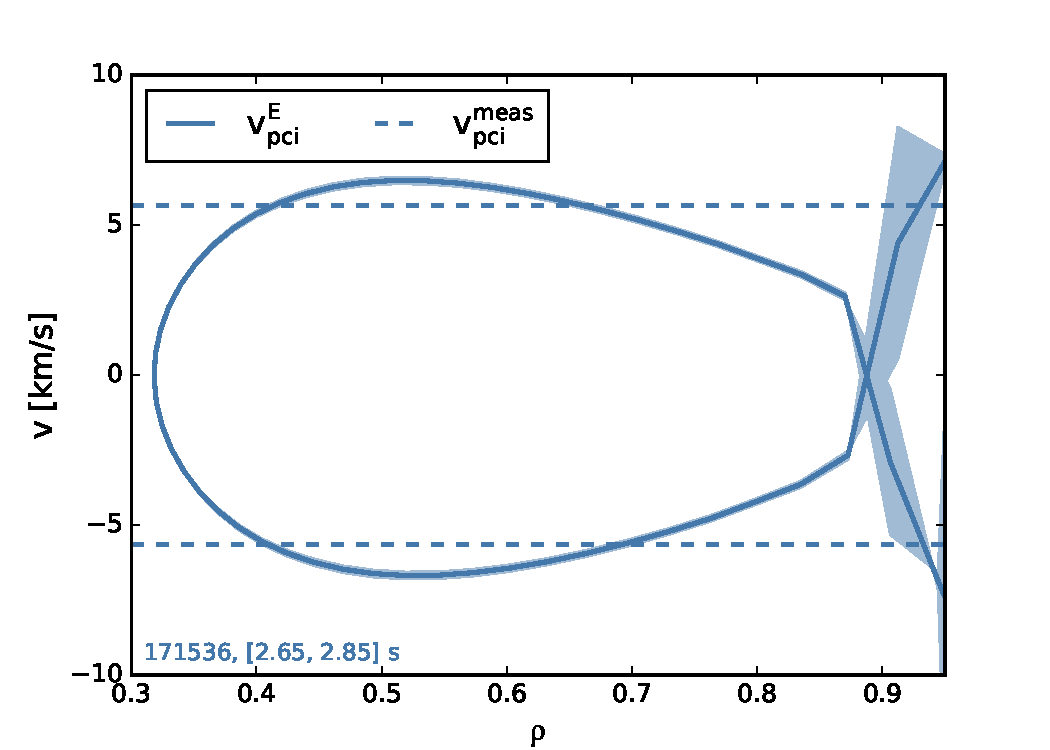
\includegraphics[width = \textwidth]{%
    Chapters/TurbulenceMeasurements/figs/doppler_shift.pdf}
  \caption[Doppler shift]{%
    Doppler shift. Positive \& negative values of $v_{\text{pci}}$
    correspond to above \& below the midplane, respectively.
    As the mask was not used, we cannot determine whether or not
    $v_{\text{meas}}$ corresponds to above or below the midplane, however
    (hence we plot $\pm v_{\text{meas}}$).
  }
\label{fig:TurbulenceMeasurements:doppler_shift}
\end{figure}

\begin{figure}[h!]
  \centering
  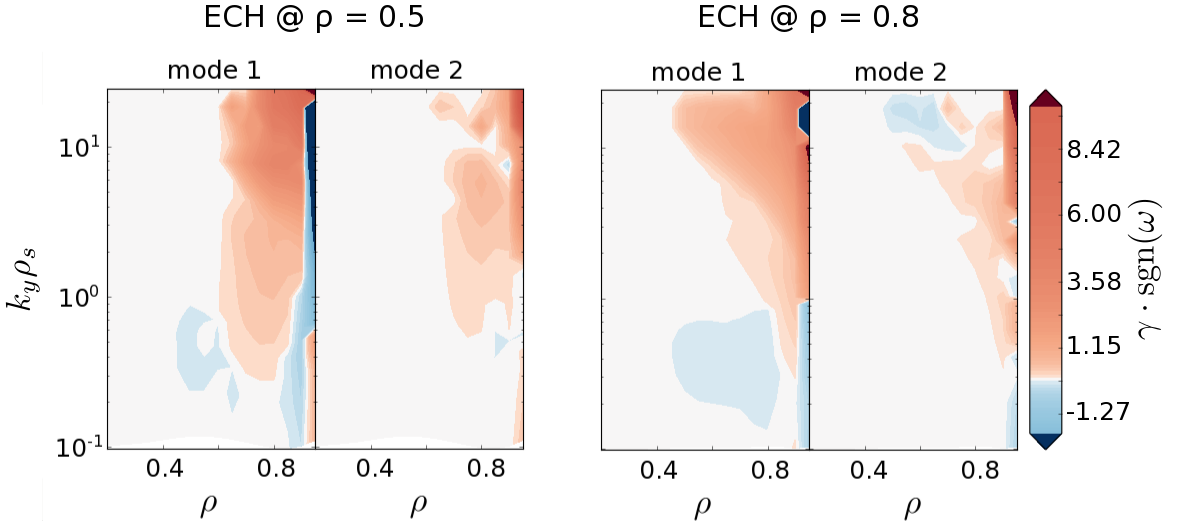
\includegraphics[width = \textwidth]{%
    Chapters/TurbulenceMeasurements/figs/TGLF_171536_vs_171538.png}
  \caption[Qualitative presentation of TGLF results]{%
    Qualitative presentation of TGLF results.
  }
\label{fig:TurbulenceMeasurements:TGLF_171536_vs_171538}
\end{figure}

\begin{figure}[h!]
  \centering
  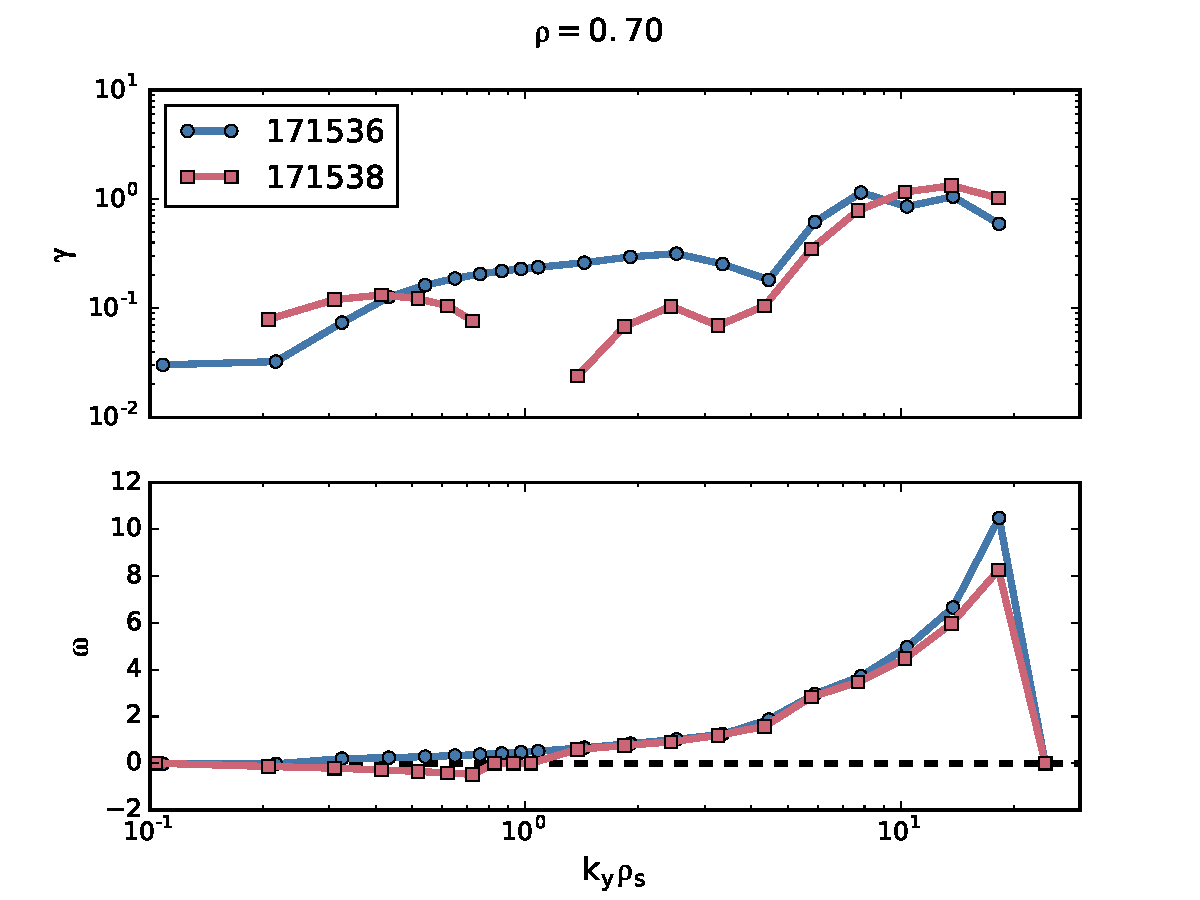
\includegraphics[width = \textwidth]{%
    Chapters/TurbulenceMeasurements/figs/linear_stability.pdf}
  \caption[Growth rates \& frequencies at $\rho=0.7$]{%
    Growth rates \& frequencies at $\rho=0.7$
    (i.e.\ we're slicing
    Figure~\ref{fig:TurbulenceMeasurements:TGLF_171536_vs_171538}
    at $\rho = 0.7$ for the most unstable mode, mode $1$).
    Note that only $171536$ uses SAT\_RULE $= 1$,
    which is calibrated against multiscale GYRO results;
    $171538$ uses SAT\_RULE $= 0$.
    Thus, it is difficult to draw conclusions\ldots
  }
\label{fig:TurbulenceMeasurements:linear_stability}
\end{figure}

\begin{figure}[h!]
  \centering
  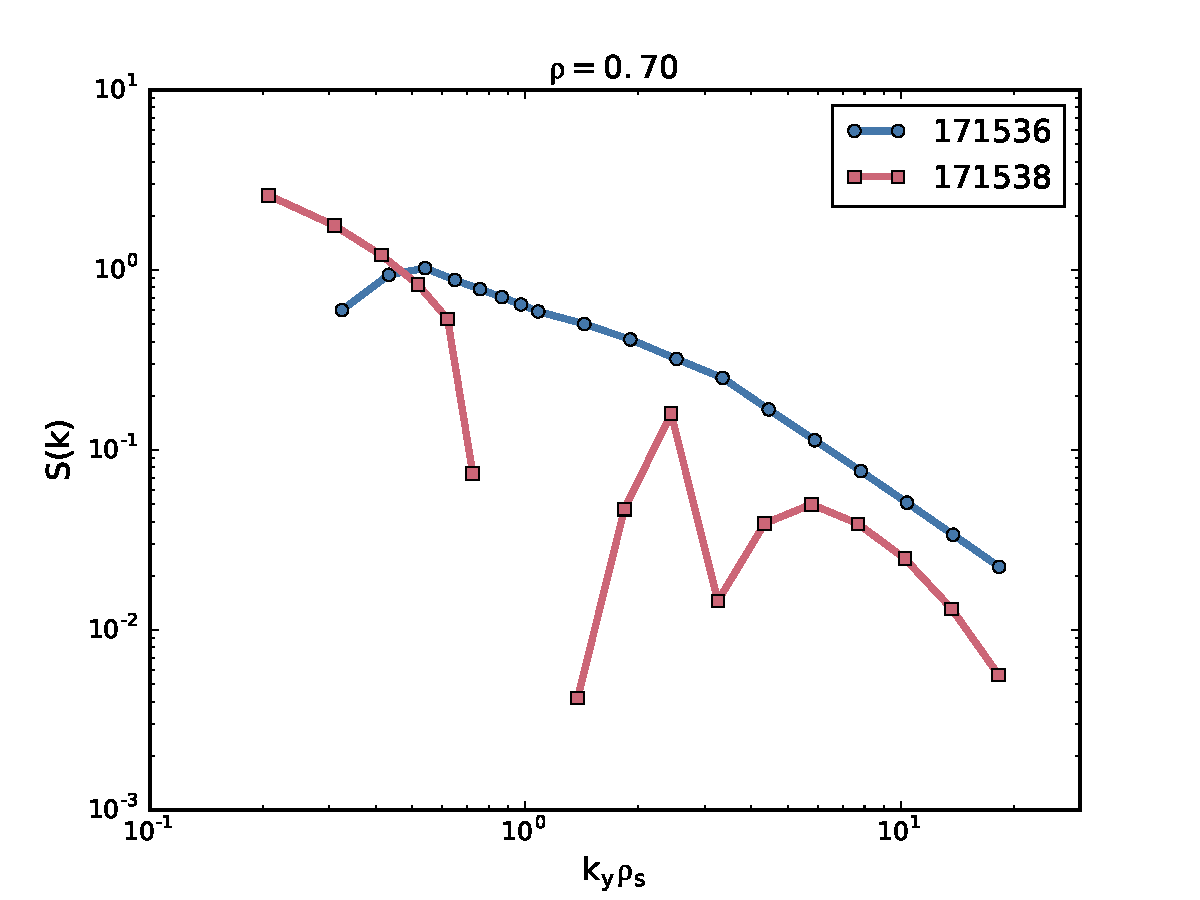
\includegraphics[width = \textwidth]{%
    Chapters/TurbulenceMeasurements/figs/density_spectra.pdf}
  \caption[TGLF-predicted density-fluctuation spectra at $\rho=0.7$]{%
    TGLF-predicted density-fluctuation spectra at $\rho=0.7$.
    Note that only $171536$ uses SAT\_RULE $= 1$,
    which is calibrated against multiscale GYRO results;
    $171538$ uses SAT\_RULE $= 0$.
    Thus, it is difficult to draw conclusions\ldots
  }
\label{fig:TurbulenceMeasurements:density_spectra}
\end{figure}


\bibliographystyle{plainurl}
\bibliography{references}
